\newcommand\pgfmathsinandcos[3]{%
  \pgfmathsetmacro#1{sin(#3)}%
  \pgfmathsetmacro#2{cos(#3)}%
}

\newcommand\LongitudePlane[3][current plane]{%
  \pgfmathsinandcos\sinEl\cosEl{#2} % elevation
  \pgfmathsinandcos\sint\cost{#3} % azimuth
  \tikzset{#1/.estyle={cm={\cost,\sint*\sinEl,0,\cosEl,(0,0)}}}
}

\newcommand\LatitudePlane[3][current plane]{%
  \pgfmathsinandcos\sinEl\cosEl{#2} % elevation
  \pgfmathsinandcos\sint\cost{#3} % latitude
  \pgfmathsetmacro\yshift{\cosEl*\sint}
  \tikzset{#1/.estyle={cm={\cost,0,0,\cost*\sinEl,(0,\yshift)}}} %
}

\newcommand\DrawLongitudeCircle[2][1]{
  \LongitudePlane{\angEl}{#2}
  \tikzset{current plane/.prefix style={scale=#1}}
   % angle of "visibility"
  \pgfmathsetmacro\angVis{atan(sin(#2)*cos(\angEl)/sin(\angEl))} %
  \draw[current plane,thin,black] (\angVis:1) arc (\angVis:\angVis+180:1);
  \draw[current plane,thin,dashed] (\angVis-180:1) arc (\angVis-180:\angVis:1);
}%this is fake: for drawing the grid


\newcommand\DrawLongitudeCirclered[2][1]{
  \LongitudePlane{\angEl}{#2}
  \tikzset{current plane/.prefix style={scale=#1}}
   % angle of "visibility"
  \pgfmathsetmacro\angVis{atan(sin(#2)*cos(\angEl)/sin(\angEl))} %
  \draw[current plane,red,thick] (150:1) arc (150:180:1);
  %\draw[current plane,dashed] (-50:1) arc (-50:-35:1);
}%for drawing the grid


\newcommand\DLongredd[2][1]{
  \LongitudePlane{\angEl}{#2}
  \tikzset{current plane/.prefix style={scale=#1}}
   % angle of "visibility"
  \pgfmathsetmacro\angVis{atan(sin(#2)*cos(\angEl)/sin(\angEl))} %
  \draw[current plane,black,dashed, ultra thick] (150:1) arc (150:180:1);
}


\newcommand\DLatred[2][1]{
  \LatitudePlane{\angEl}{#2}
  \tikzset{current plane/.prefix style={scale=#1}}
  \pgfmathsetmacro\sinVis{sin(#2)/cos(#2)*sin(\angEl)/cos(\angEl)}
  % angle of "visibility"
  \pgfmathsetmacro\angVis{asin(min(1,max(\sinVis,-1)))}
  \draw[current plane,dashed,black,ultra thick] (-50:1) arc (-50:-35:1);
}


\newcommand\fillred[2][1]{
  \LongitudePlane{\angEl}{#2}
  \tikzset{current plane/.prefix style={scale=#1}}
   % angle of "visibility"
  \pgfmathsetmacro\angVis{atan(sin(#2)*cos(\angEl)/sin(\angEl))} %
  \draw[current plane,red,thin] (\angVis:1) arc (\angVis:\angVis+180:1);
}

\newcommand\DrawLatitudeCircle[2][1]{
  \LatitudePlane{\angEl}{#2}
  \tikzset{current plane/.prefix style={scale=#1}}
  \pgfmathsetmacro\sinVis{sin(#2)/cos(#2)*sin(\angEl)/cos(\angEl)}
  % angle of "visibility"
  \pgfmathsetmacro\angVis{asin(min(1,max(\sinVis,-1)))}
  \draw[current plane,thin,black] (\angVis:1) arc (\angVis:-\angVis-180:1);
  \draw[current plane,thin,dashed] (180-\angVis:1) arc (180-\angVis:\angVis:1);
}%Defining functions to draw limited latitude circles (for the red mesh)


\newcommand\DrawLatitudeCirclered[2][1]{
  \LatitudePlane{\angEl}{#2}
  \tikzset{current plane/.prefix style={scale=#1}}
  \pgfmathsetmacro\sinVis{sin(#2)/cos(#2)*sin(\angEl)/cos(\angEl)}
  % angle of "visibility"
  \pgfmathsetmacro\angVis{asin(min(1,max(\sinVis,-1)))}
  %\draw[current plane,red,thick] (-\angVis-50:1) arc (-\angVis-50:-\angVis-20:1);
\draw[current plane,red,thick] (-50:1) arc (-50:-35:1);
}


\tikzset{
  >=latex,
  inner sep=0pt,
  outer sep=2pt,
  mark coordinate/.style={inner sep=0pt,outer sep=0pt,minimum size=3pt, fill=black,circle}
}


\section{Aufgabe 1 \& 2 - Orthodromie}
%\subsection{Aufgabenstellung}
%\begin{itemize}
  %\item Erstellung eines Entscheidungsnetzes auf der Erdkugel
  %\item Berechnung einer Orthodromie (Distanz in Meilen zwischen zwei Punkten auf der Erdkugel)
  %\item Erstellung der Koordinatendatei eines Sees
%\end{itemize}

\subsection{Analyse der Problemstellung}
\subsubsection{Berechnung einer Orthodromie}
Auf einer Kugel soll zwischen zwei Punkten die kürzeste Route bzw. die kürzeste Verbindung gewählt werden, welche auch Orthodrome genannt wird. Die Orthodrome ist immer ein Teilstück eines grossen Kreises. Um die kürzeste Verbindung zwischen den beiden Punkten $A$ und $B$ zu berechnen, werden zuerst die beiden Vektoren vom Kugelursprung bis zu den Punkten ermittelt. Die beiden Vektoren spannen dann mit dem Ursprung eine Ebene auf, deren Schnittlinie mit der Kugeloberfläche (Sphäre) die Orthodrome darstellt. Da die zwei Punkte den Kreis in zwei Kreisbogen separieren, wird nur der kürzere Distanz berücksichtigt.


Auf der Erdoberfläche werden die zwei Punkten in geographische Koordinaten, Längen- und Breitengrad, angegeben. Die Erde wird dabei in 360 Längengrade und 180 Breitengrade aufgeteilt. Somit haben die beiden Punkte die folgende Struktur: $A$ (\(\theta_1 , \phi_1\)) und $B$ (\(\theta_2 , \phi_2\)).

Für die Berechnung der Distanz benötigen wir die Längen- und Breitengrade der zwei Punkte in Radian, welche dann in die Formel \eqref{eq:1} wie folgt eingesetzt werden: \\
% Formel ArcCos(...)
\begin{equation}
\label{eq:1}
 \frac{360*60}{2 \pi} \arccos[\cos(\theta_1 - \theta_2) \cos(\phi_1) \cos(\phi_2)+\sin(\phi_1) \sin(\phi_2)]
 \end{equation}


%Die aufgespaltete Ebene lässt sich mit dem Vektorprodukt der beiden Punkten $A$ und $B$  berechnen. 


%Da die Erde eine Kugelform hat, werden die Koordinaten in Längen- und Breitengraden und die Distanz in Seemeilen angegeben. 

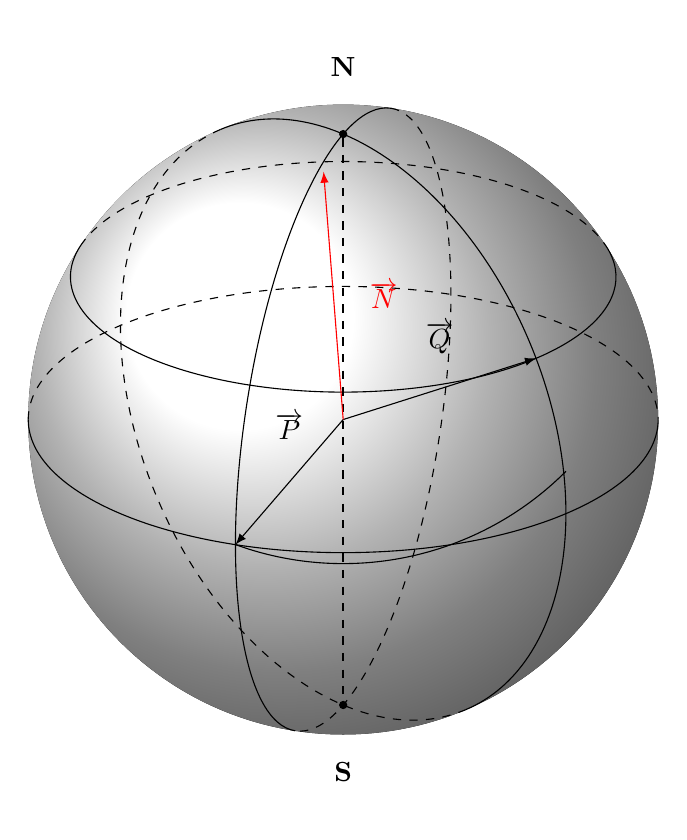
\begin{tikzpicture}[scale=1,every node/.style={minimum size=1cm}]
	%% some definitions
	
	\def\R{4} % sphere radius
	
	\def\angEl{25} % elevation angle
	\def\angAz{-100} % azimuth angle
	\def\angPhiOne{-110} % longitude of point P
	\def\angPhiTwo{-45} % longitude of point Q
	\def\angBeta{30} % latitude of point P and Q
	
	%% working planes
	
	\pgfmathsetmacro\H{\R*cos(\angEl)} % distance to north pole
	\LongitudePlane[xzplane]{\angEl}{\angAz}
	\LongitudePlane[pzplane]{\angEl}{\angPhiOne}
	\LongitudePlane[qzplane]{\angEl}{\angPhiTwo}
        \LongitudePlane[nzplane]{\angEl}{-86}
	\LatitudePlane[equator]{\angEl}{0}
	\fill[ball color=white!10] (0,0) circle (\R); % 3D lighting effect
	\coordinate (O) at (0,0);
	\coordinate[mark coordinate] (N) at (0,\H);
	\coordinate[mark coordinate] (S) at (0,-\H);
	
    \DrawLongitudeCircle[\R]{\angPhiOne} % pzplane
    \DrawLongitudeCircle[\R]{\angPhiTwo} % qzplane
    \DrawLatitudeCircle[\R]{\angBeta}
    \DrawLatitudeCircle[\R]{0} % equator
	%labelling north and south
	\node[above=8pt] at (N) {$\mathbf{N}$};
	\node[below=8pt] at (S) {$\mathbf{S}$};
        \draw[-,dashed, thick] (N) -- (S);

    %setup coordinates P and Q
    \path[pzplane] (0:\R) coordinate (P);
    \draw[->] (O) -- node[above=4pt] {$\overrightarrow{P}$} (P);
    \path[qzplane] (\angBeta:\R) coordinate (Q);
    \draw[->] (O) -- node[above=2pt] {$\overrightarrow{Q}$} (Q);
    \path[nzplane] (153:\R) coordinate (N);
    \draw[->,color=red] (O) -- node[right=2pt] {$\overrightarrow{N}$} (N);
    \draw (P) arc (-110:-45:\R) (Q);	
\end{tikzpicture}

\subsubsection{Erstellung eines Entscheidungsnetzes auf der Erdkugel}
Es soll ein Koordinatennetz mit den Knoten erstellt werden, auf welches dann später die Berechnungen durchgeführt werden. Für die Erstellung des Netzes benötigt man den Start- und Endpunkt als Eingabe. Die Anzahl der Knoten im Netz werden von den weiteren zwei Eingaben m und n definiert, wobei m für die Anzahl der Spalten und n für die Anzahl der Zeilen steht. Alle Punkte in diesem Netz beinhalten ihre eigene Informationen über das Längen- und Breitengrad.

Der Abstand zwischen dem Start- und Endpunkt wird mittels der Euklidischen-Abstand Verfahren ermittelt. Die Formel dafür lautet:
\begin{equation}
\label{eq:2}
e = \sqrt{ (\theta_2 - \theta_1)^2 + (\phi_2-\phi_1)^2}
 \end{equation}
Somit sind die Spaltenlänge durch e/m und die Zeilenhöhe durch e/n definiert. Da der Graph auch rotiert werden kann, braucht es eine Rotations-Matrix, welches sich wie folgt zusammensetzt.
\begin{equation}
\label{eq:3}
M = \begin{pmatrix} \frac{\theta_2 - \theta_1}{e} & \frac{\phi_2 - \phi_1}{e} \\ \frac{\phi_2 - \phi_1}{e} & \frac{\theta_2 - \theta_1}{e} \end{pmatrix}
 \end{equation}
 

